\section{Factorial analysis on different number of nodes}
The purpose of this section is to confront the results of the factorial analysis for various models with different number of nodes, since the process for obtaining these results is the same explained in section \ref{sec:ModelFitting}, we shall skip directly to the values for influences and comment them.
\subsection{Influence on coverage rate and time}
We first analyze the result for the coverage percentage and the coverage time.

\begin{table}[H]
\centering
\begin{tabular}{|c|l|l|l|}
\hline
\textbf{Number of nodes} & \multicolumn{1}{c|}{\textbf{Probability}} & \multicolumn{1}{c|}{\textbf{Radius}} & \multicolumn{1}{c|}{\textbf{Combined}} \\ \hline
\textbf{50} & 0,00206 & 0,996125 & 0,001816 \\ \hline
\textbf{100} & 0,005405 & 0,993859 & 0,000736 \\ \hline
\textbf{200} & 0,403551 & 0,447621 & 0,148828 \\ \hline
\textbf{500} & 0,904792 & 0,046432 & 0,048775 \\ \hline
\textbf{700} & 0,95802 & 0,020789 & 0,021191 \\ \hline
\end{tabular}
\caption{Influence for the coverage percentage}
\end{table}

\begin{table}[H]
\centering
\begin{tabular}{|c|l|l|l|}
\hline
\multicolumn{1}{|l|}{\textbf{Number of nodes}} & \multicolumn{1}{c|}{\textbf{Probability}} & \multicolumn{1}{c|}{\textbf{Radius}} & \multicolumn{1}{c|}{\textbf{Combined}} \\ \hline
\textbf{50} & 0,826853 & 0,11478 & 0,058367 \\ \hline
\textbf{100} & 0,981894 & 0,010828 & 0,007278 \\ \hline
\textbf{200} & 0,667182 & 0,237209 & 0,09561 \\ \hline
\textbf{500} & 0,957135 & 0,033649 & 0,009216 \\ \hline
\textbf{700} & 0,96461 & 0,00596 & 0,029431 \\ \hline
\end{tabular}
\caption{Influence for the coverage time}
\end{table}

To draw easier conclusion, in the following section, these result are plotted in a scatter plot with lines.

\begin{figure}[H]\label{pic:CovPerc}
\centering
    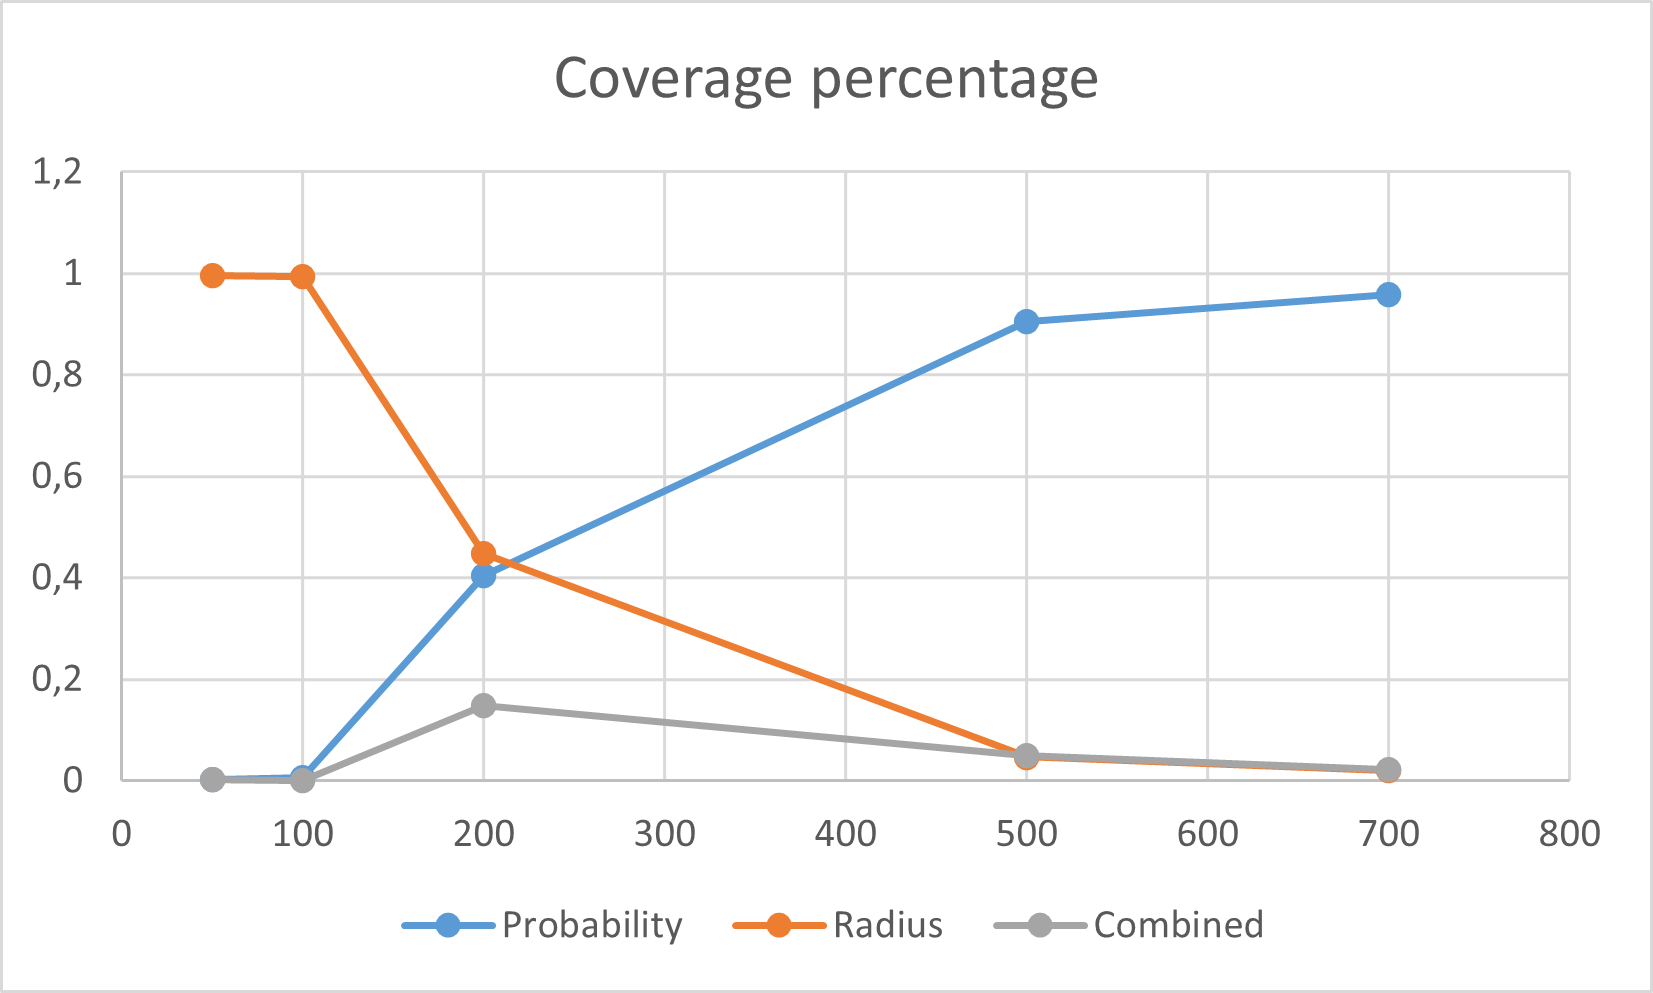
\includegraphics[width= 1\textwidth]{./images/CoveragePercentageWithNodes.png}
    \caption{Coverage percentage at different nodes}
    \label{fig:immagine}
\end{figure}


\begin{figure}[H]
\centering
    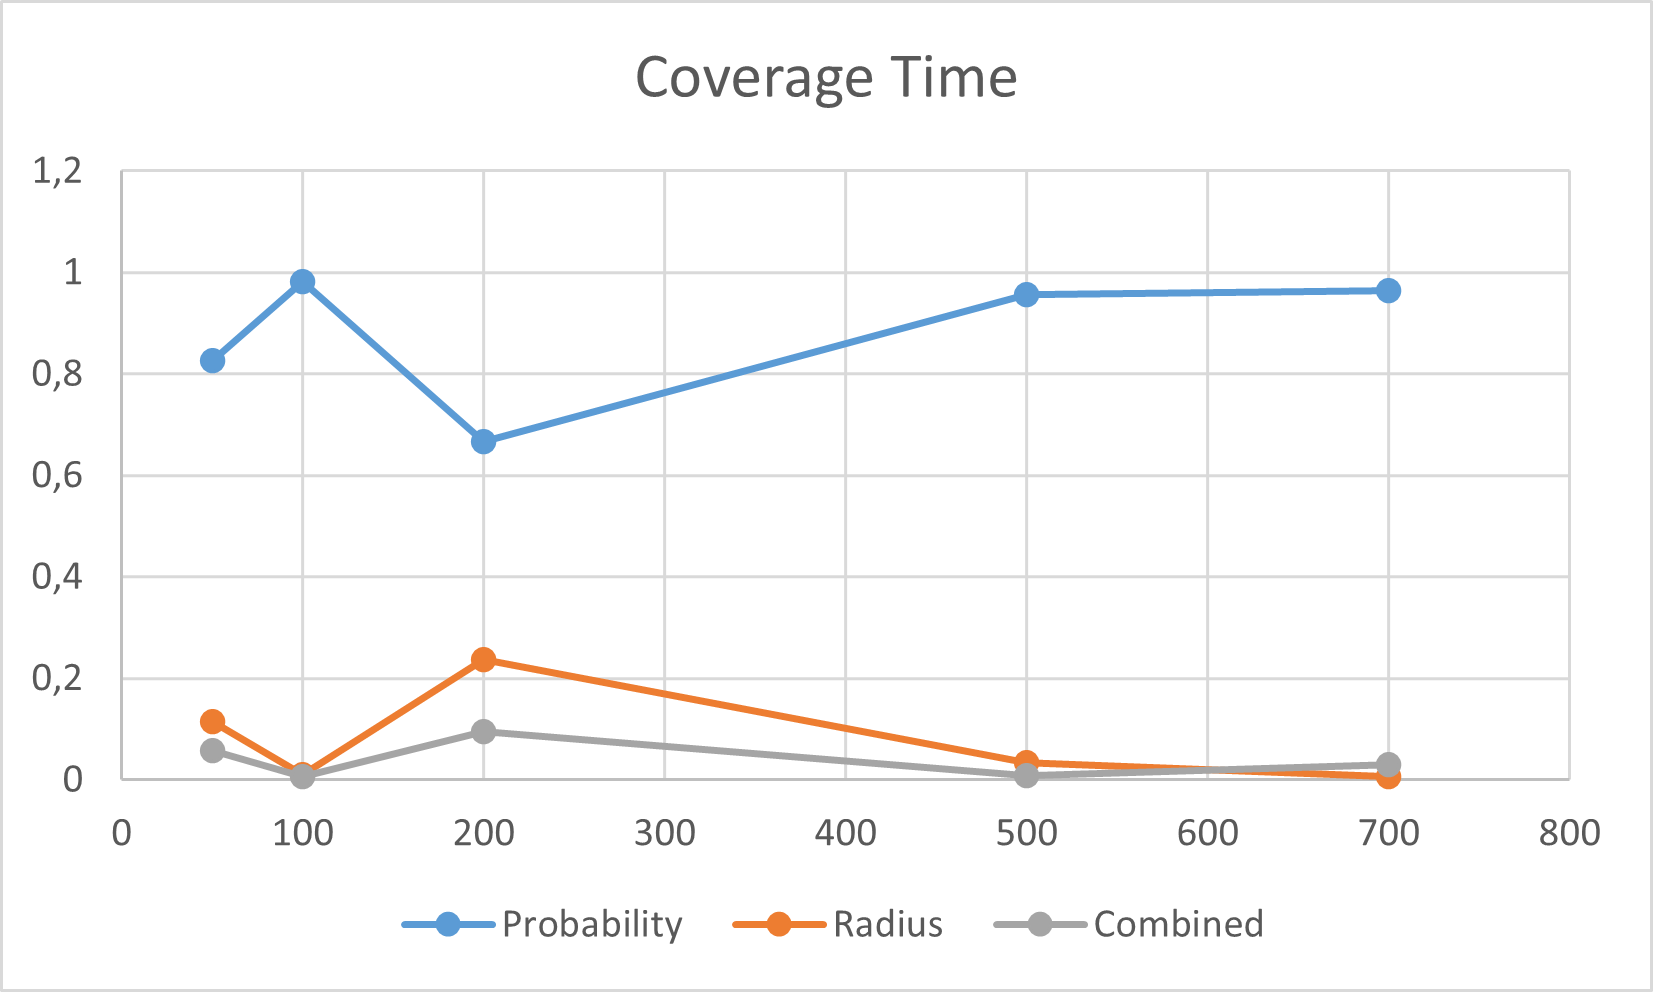
\includegraphics[width= 1\textwidth]{./images/CoverageTimeWithNodes.png}
    \caption{Coverage time at different nodes}
    \label{fig:immagine}
\end{figure}

Let's start with \ref{pic:CovPerc} it is easy to understand that a low density the radius is far more critical then the probability since with low radius it is likely that many nodes are isolated or do not get a second "chance" after receiving a collision. At high number of nodes, the contrary happens the reason of this behavior is that even with low radius each node as a lot of neighbors so it is far more important for them to be able to easily transmit.

The coverage time is more tricky to understand, with a high number of nodes it is far more important for the nodes to quickly transmit for same motivation previously stated. However with a low density the behavior for the influences is more chaotic, this happens because, since this analysis takes account only for the coverage time, some runs end immediately with a high probability and low radius however these configuration result in a very low coverage percentage. With 200 nodes a critical point is reached the reason behind is that this configuration have a high enough density for the runs to not immediately terminate as in the previous cases, this result in a still high influence for the probability factor due to the same reason explained for configuration with high number of node, but still gains for a higher radius so that more nodes are reached at each transmission.

\subsection{Analysis on the models parameter}
The next step is to perform the same confrontation for the models parameters, obviously the Gompertz model is used since it was already concluded to be the most fitting one

\begin{table}[H]
\centering
\begin{tabular}{|c|c|c|c|}
\hline
\textbf{Number} & \textbf{Probability} & \textbf{Radius} & \textbf{Combined} \\ \hline
\textbf{50} & 0,002001 & 0,996207 & 0,001792 \\ \hline
\textbf{100} & 0,005439 & 0,993876 & 0,000685 \\ \hline
\textbf{200} & 0,409502 & 0,436643 & 0,153855 \\ \hline
\textbf{500} & 0,899014 & 0,057842 & 0,043144 \\ \hline
\textbf{700} & 0,951368 & 0,0317 & 0,016932 \\ \hline
\end{tabular}
\caption{Influence for the asymptote}
\end{table} 


\begin{table}[H]
\centering
\begin{tabular}{|c|l|l|l|}
\hline
\textbf{Number} & \multicolumn{1}{c|}{\textbf{Probability}} & \multicolumn{1}{c|}{\textbf{Radius}} & \multicolumn{1}{c|}{\textbf{Combined}} \\ \hline
\textbf{50} & \multicolumn{1}{c|}{0,232476} & 0,057973 & 0,709551 \\ \hline
\textbf{100} & 0,549222 & 0,309554 & 0,141225 \\ \hline
\textbf{200} & 0,066563 & 0,901042 & 0,032395 \\ \hline
\textbf{500} & 0,002461 & 0,985123 & 0,012416 \\ \hline
\textbf{700} & 0,001625 & 0,990217 & 0,008158 \\ \hline
\end{tabular}
\caption{Influence for the displacement}
\end{table}


\begin{table}[H]
\centering
\begin{tabular}{|c|c|c|c|}
\hline
\textbf{Number} & \textbf{Probability} & \textbf{Radius} & \textbf{Combined} \\ \hline
\textbf{50} & 0,944422 & 0,002066 & 0,053511 \\ \hline
\textbf{100} & 0,36719 & 0,346769 & 0,286041 \\ \hline
\textbf{200} & 0,557802 & 0,379108 & 0,06309 \\ \hline
\textbf{500} & 0,904364 & 0,028022 & 0,067614 \\ \hline
\textbf{700} & 0,958562 & 0,011033 & 0,030405 \\ \hline
\end{tabular}
\caption{Influence for the growth rate}
\end{table}

As previously done the same kind of scatter plot is shown underneath to better understand the patterns.

\begin{figure}[H]\label{pic:AsymptoteNodes}
\centering
    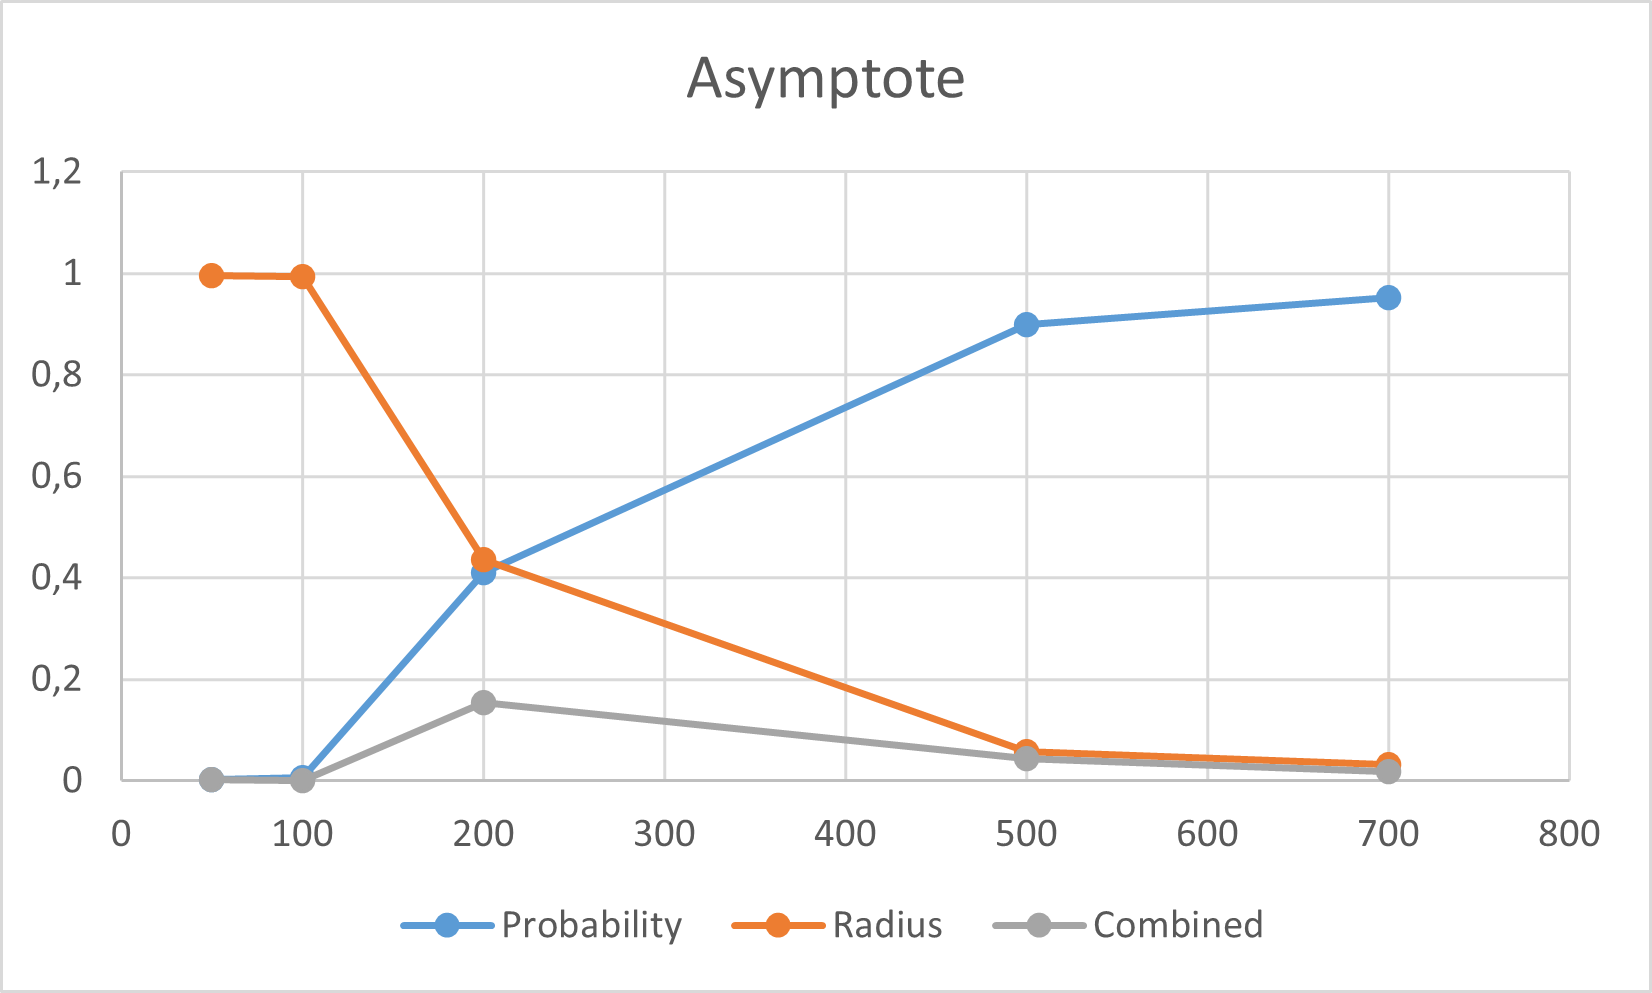
\includegraphics[width= 1\textwidth]{./images/AsymptoteWithNodes.png}
    \caption{Asymptote influences at different nodes}

\end{figure}

As expected the influences for the asymptote are similar to the one for the coverage percentage, so it is unnecessary to repeat the same explanation.

\begin{figure}[H]\label{pic:DisplacementNodes}
\centering
    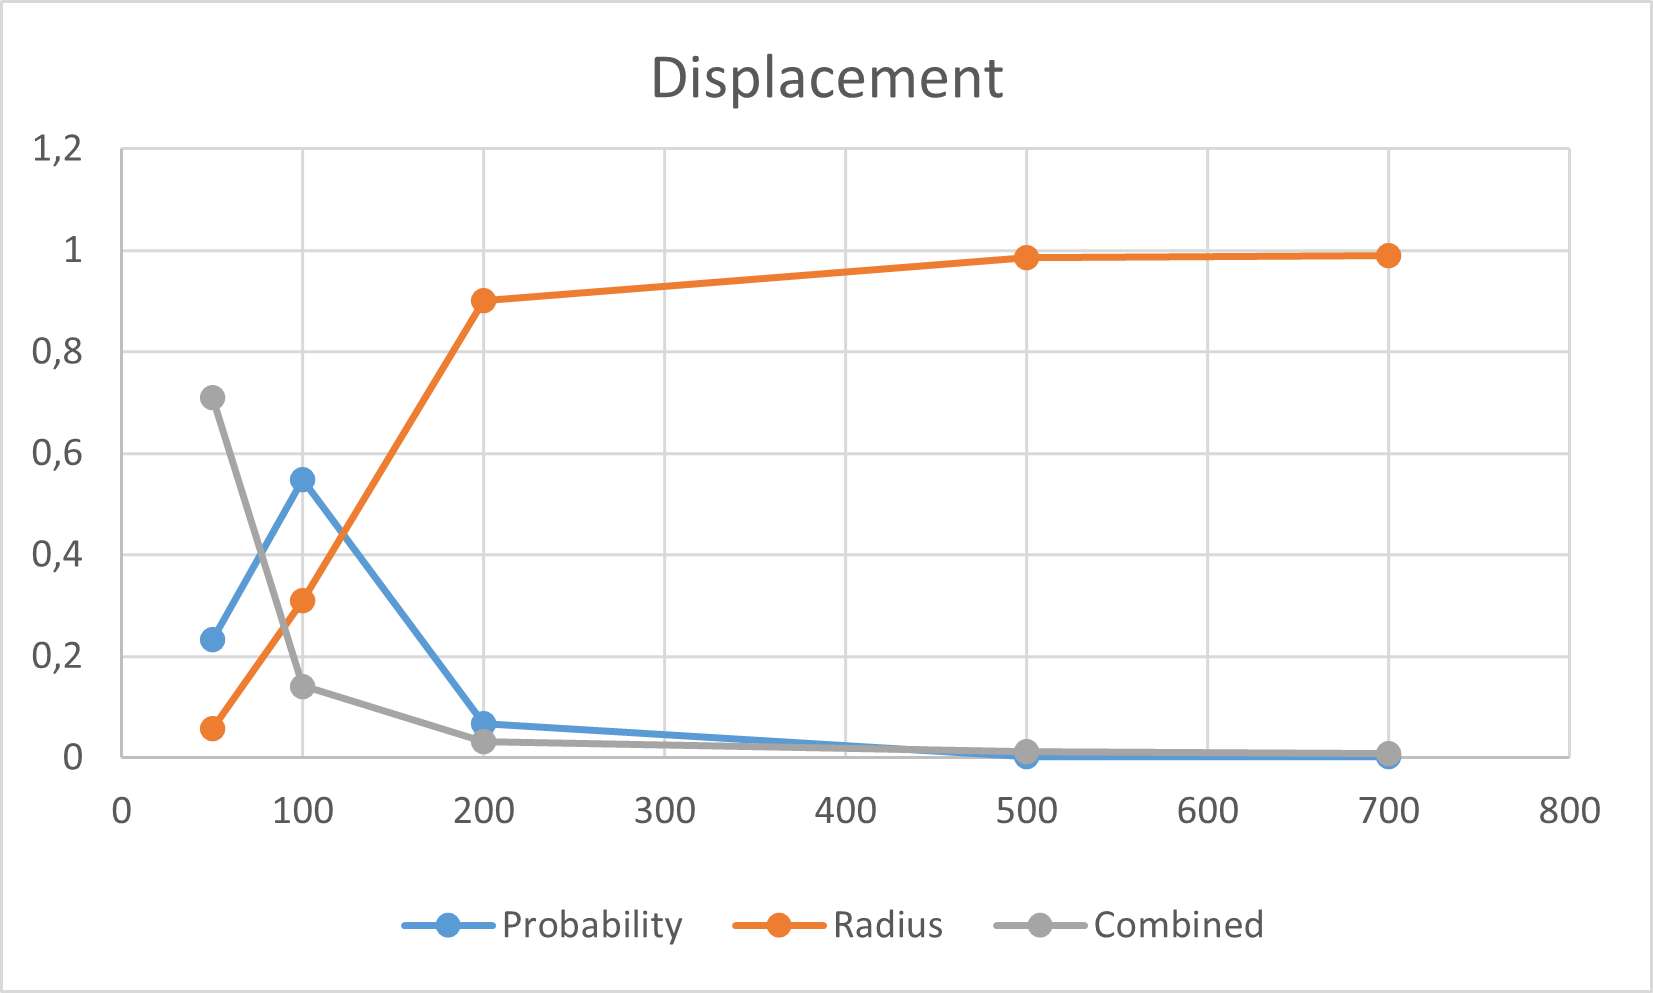
\includegraphics[width= 1\textwidth]{./images/DisplacementWithNodes.png}
    \caption{Displacement influences at different nodes}
\end{figure}

At low density to achieve a high displacement it is necessary to have a high combined effort so that the patient zero node have many neighbor and so that they can transmit immediately due to a high probability. With a growing density the radius influence takes up with a "quantity over quality" logic where, even with low probability, a high radius allow the first infected node to reach a great number of nodes, generating a high displacement even if some nodes do not immediately re-transmit.

\begin{figure}[H]\label{pic:GrowthRatesNodes}
\centering
    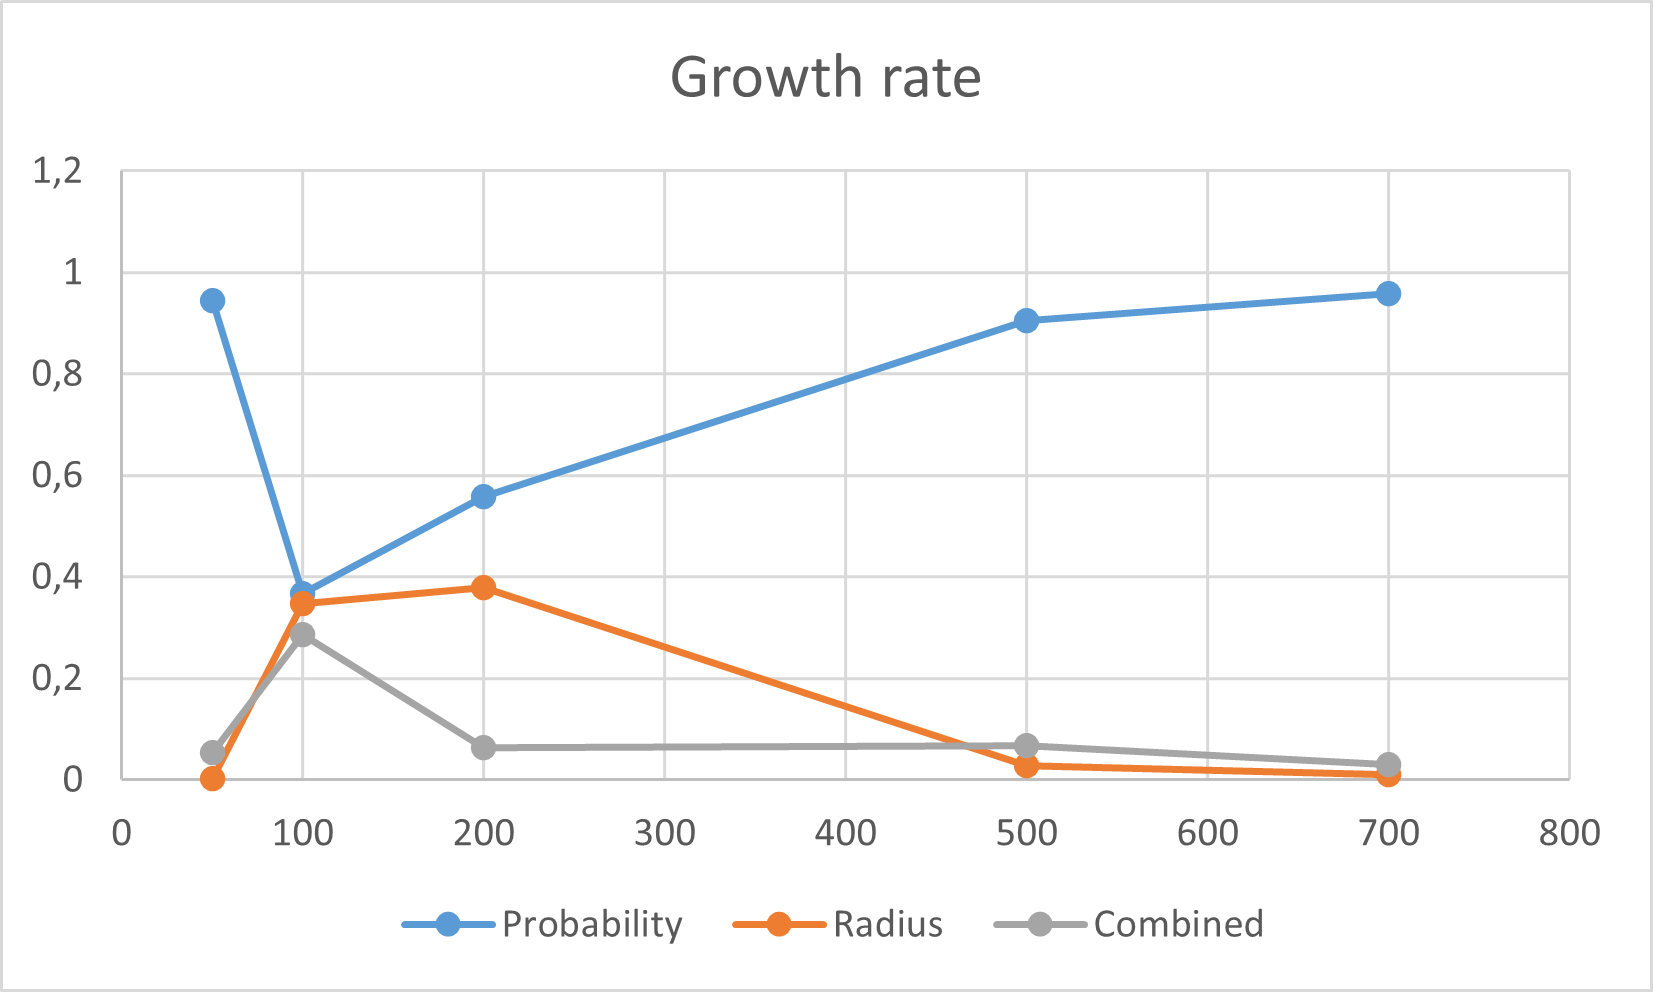
\includegraphics[width= 1\textwidth]{./images/GrowthRateWithNodes.png}
    \caption{Growth rate influences at different nodes}
\end{figure}

The growth rate 